%%%%%%%%%%%%%%%%%%%%%%%%%%%%%%%%%%%%%%%%%
% Journal Article
% LaTeX Template
% Version 1.3 (9/9/13)
%
% This template has been downloaded from:
% http://www.LaTeXTemplates.com
%
% Original author:
% Frits Wenneker (http://www.howtotex.com)
%
% License:
% CC BY-NC-SA 3.0 (http://creativecommons.org/licenses/by-nc-sa/3.0/)
%
%%%%%%%%%%%%%%%%%%%%%%%%%%%%%%%%%%%%%%%%%

%----------------------------------------------------------------------------------------
%	PACKAGES AND OTHER DOCUMENT CONFIGURATIONS
%----------------------------------------------------------------------------------------

\documentclass[twoside]{article}

\usepackage{lipsum} % Package to generate dummy text throughout this template

\usepackage{amsmath,amsthm,amssymb}

\usepackage[hmarginratio=1:1,top=32mm,columnsep=20pt]{geometry} % Document margins
\usepackage{multicol} % Used for the two-column layout of the document
\usepackage[hang, small,labelfont=bf,up,textfont=it,up]{caption} % Custom captions under/above floats in tables or figures
\usepackage{booktabs} % Horizontal rules in tables
\usepackage{float} % Required for tables and figures in the multi-column environment - they need to be placed in specific locations with the [H] (e.g. \begin{table}[H])
\usepackage{hyperref} % For hyperlinks in the PDF
\usepackage[export]{adjustbox}
%\usepackage{subcaption}


\usepackage{paralist} % Used for the compactitem environment which makes bullet points with less space between them

\usepackage{abstract} % Allows abstract customization
\renewcommand{\abstractnamefont}{\Large\normalfont\bfseries} % Set the "Abstract" text to bold
%\renewcommand{\abstracttextfont}{\normalfont\small\itshape} % Set the abstract itself to small italic text

\usepackage{titlesec} % Allows customization of titles
\titleformat{\section}[block]{\Large\bf\scshape\centering}{\thesection.}{0.25em}{} % Change the look of the section titles
%\titleformat{\subsection}[block]{\large}{\thesubsection.}{1em}{} % Change the look of the section titles

\usepackage{fancyhdr} % Headers and footers
\usepackage{graphicx}
\usepackage{wrapfig}
\usepackage{subfig}
\usepackage{cancel}
\usepackage[normalem]{ulem}

%\pagestyle{fancy} % All pages have headers and footers
%\fancyhead{} % Blank out the default header
%\fancyfoot{} % Blank out the default footer
%\fancyhead[C]{Running title $\bullet$ November 2012 $\bullet$ Vol. XXI, No. 1} % Custom header text
%\fancyfoot[RO,LE]{\thepage} % Custom footer text

%----------------------------------------------------------------------------------------
%	TITLE SECTION
%----------------------------------------------------------------------------------------

\title{\vspace{-15mm}\fontsize{20pt}{10pt}\selectfont\textbf{Comparison of Time-Stepping methods for late times EM diffusion phenomenons in Geophysics}} % Article title
\author{
\Large
\textsc{Math 607E: Course Project}
\\\\
\large
\textsc{Thibaut Astic}\\%Or \normalsize for text
\textsc{90142150} \\ % Your institution
\normalsize thast@eos.ubc.ca
\vspace{-5mm}
}
\date{}

%----------------------------------------------------------------------------------------

\begin{document}

\maketitle % Insert title

%\thispagestyle{fancy} % All pages have headers and footers

%----------------------------------------------------------------------------------------
%	ABSTRACT
%----------------------------------------------------------------------------------------

\begin{abstract}

In mineral resources exploration, Time-Domain Electromagnetic (TDEM) data are acquired to image conductive structures in the subsurface. A widely used setup measures the response to a step-off electric current in an inductive loop in term either of the magnetic flux density ${\bf b}_z$ of its first derivative $\frac{\partial {\bf b}_z}{\partial t}$ , with the loop and receiver either in the air or at the surface. The receiver is generally placed at the center of the loop to avoid side effects, as described in \cite{WH:1988}. Electromagnetic phenomenons are described by Maxwell's equations, whose forms a complex system of partial differential equations linking fields and fluxes. We use a finite volume discretization to solve these equations, because of its conservation of mass property. At $t\leq 0$, the fields are static and can be computed in various ways. We discuss how diverse initializations can lead to different accuracy behaviors later in time. At $t>0$, Maxwell's equations are well-known to be very stiff (\cite{HAO:2004}), requiring the use of implicit time-stepping methods. Moreover, the physical system displays wave behaviors at very early time channels we do not want to compute for later diffusive time windows. We test different time-stepping methods and compare their accuracy to an exact analytic solution. Backward Euler has appeared to be very reliable and stable but can require a lot of steps to give an accurate solution at late times. We encounter some issues to do a proper convergence analysis of BDF-2. Its behavior has proven to be highly sensitive to our mesh. However it has consistently displays better accuracy at late times than Backward Euler and in a lower number of time-steps for a comparable cost. BDF-4 has been briefly tested but the lose of A-stability seems to add to the previous problems encounter in BDF-2. 


\end{abstract}

%----------------------------------------------------------------------------------------
%	ARTICLE CONTENTS
%----------------------------------------------------------------------------------------

%\begin{multicols}{2} % Two-column layout throughout the main article text

\section{Introduction}
Characterizing the Earth's subsurface is one of the key questions in Earth Sciences, either to image the Earth's core, anticipating pollution migration, finding minerals resources etc. Geophysics goal is to image these structures remotely by measuring Earth's response to different fields. 

One of the main group of methods uses in Geophysics are Electromagnetic methods (\cite{WH:1988}). With this project we are going to particularly focus on Time-Domain Electromagnetic (TDEM, figure \ref{TDEM_quickdraw}) fields generated by inductive sources under diffusion assumptions. Electromagnetic phenomenons are governed by Maxwell's equations and hence are sensitive to contrasts in physical properties that can be interpreted in terms of geologic structure and fluid content. The diagnostic physical property for TDEM is electrical conductivity $\sigma$ (or its inverse resistivity $\rho$). In a nutshell, once we cut-off the current in the loop, eddy currents are generated according to Faraday's law in the ground to compensate the loss in the current loop and maintain the magnetic field. These currents are attenuated due to ohm's law, producing a change in the magnetic field, which results in induced eddy currents and so on. The final result is an downward and outward diffusion of rotational currents in the ground, commonly called `smoke rings' (\cite{Nabighian}). We can measure these changes in the magnetic field and then interpret them in term of conductivity contrasts in the subsurface (figure \ref{DecayCurves}).

\begin{figure}[!ht]
\centering
\begin{minipage}{0.5\textwidth}
  \centering
  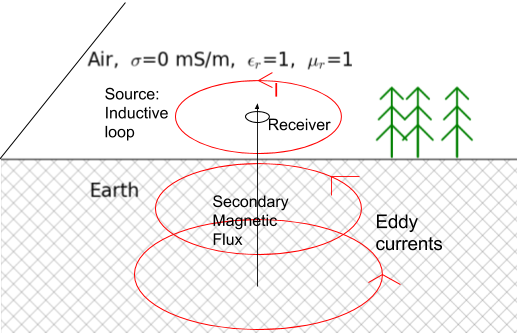
\includegraphics[width=.9\linewidth]{./figures/TDEM_quickdraw.png}
  \captionof{figure}{TDEM system in a nutshell}
  \label{TDEM_quickdraw}
\end{minipage}%
\begin{minipage}{.5\textwidth}
  \centering
  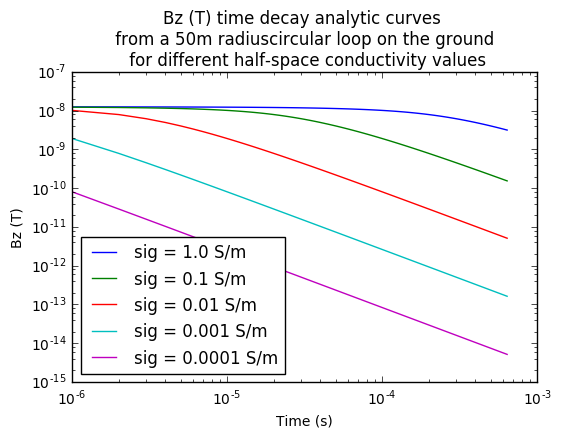
\includegraphics[width=.9\linewidth]{./figures/AnalyticCurve.png}
  \captionof{figure}{Proof of concept: decay curves for various half-space conductivity}
  \label{DecayCurves}
\end{minipage}
\end{figure}

Maxwell's equation forms a complex system of Partial Differential Equations. In most cases, there is no analytic solution except for very simple problems (half-space, sphere in void…). To forward model the response of complex structures, numerical techniques are required. We present in this project a discretization in space of our TDEM problem using staggered grid and finite volume (\cite{Haber:2014}). Using this discretization, we have tested different time stepping methods (explicit and implicit, single and multi steps) in term of cost and accuracy to compute the late times corresponding to the diffusion phenomenons and this without computing the wave part of Maxwell's equation. We then investigate if computing late times without early diffusive times can be accurate with higher order methods.This project has been realized in Python and rely on the Python open source package SimPEG developed at UBC for the mesh and matrices operators (\cite{CKH+:2015}).

Code and scripts to re-create most of the results generated for this project are available through Github at the address: 
https://github.com/thast/Math607E

%------------------------------------------------

\section{Time Domain Discretization of Maxwell's Equation Using a finite volume E-B formulation}

We start by writing Faraday's law and Ampere's law:
\begin{align}
\frac{ \partial {\bf b}}{\partial t} + \nabla \times {\bf e} &= {\bf 0} \label{Faraday} \\
\nabla \times \mu^{-1}{\bf b} - \sigma {\bf e} - \varepsilon_0 \frac{\partial {\bf e}}{\partial t} &= \bf{j_s} + \bf{j_m} + \bf{j_p} \label{Ampere}
\end{align}

In our case we assume a magneto-quasi-static state. This means we are neglecting the electric displacement current $\varepsilon_0 \frac{\partial e}{\partial t}$ and therefore the electromagnetic waves due to the coupling of the magnetic induction with the displacement current in equation \ref{Ampere}. We also ignore the magnetization current $j_m$ (ignoring magnetization of Earth's material) and polarization current $j_p$ (ignoring any polarization of Earth's material), only keeping our source term $j_s$. The usual diagnostic property for TDEM systems is the electric conductivity $\sigma$, as it usually varies a lot more than the magnetic permeability $\mu$, our model will assume that $\mu = \mu_0$ everywhere.

\begin{align}
\frac{ \partial {\bf b}}{\partial t} + \nabla \times {\bf e} &= {\bf 0} \\
\nabla \times \mu_0^{-1}{\bf b} - \sigma {\bf e} &= {\bf {j_s}} \label{Ampere_quasistatic}
\end{align}

In finite volume on a staggered grid, we assign different physical quantities to the different parts of the mesh: cell-centers, nodes, edges and faces. We choose here to discretize according to the so-called E-B formulation, in opposition with the other popular duo field-flux discretization, the H-J formulation (\cite{simpegjournal}). As shown in figure \ref{EB_formulation}, we put on cell-centers physical quantities that are consider constant over each cell, here our physical properties. As a flux and our data, the magnetic flux density is discretized on the faces. This forces the electric field to be discretized on the edges, as related to B through a curl operator. This is a convenient choice to discretize the wire of our source loop which is likely to be smaller that our cell size.

\begin{figure}[!ht]
%\vspace{-10pt}
\centering
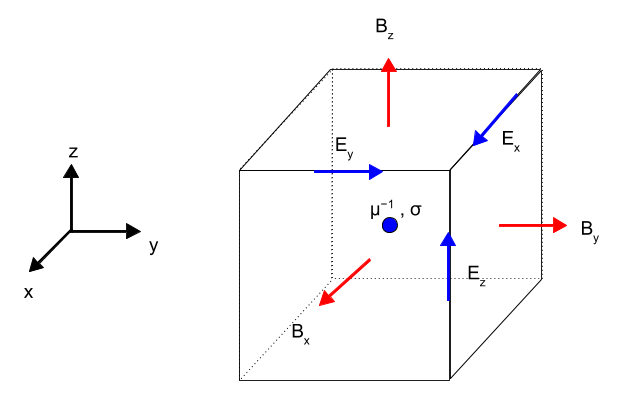
\includegraphics[scale=0.4]{./figures/EB_formulation.png}
\caption{EB Formulation: where do things live}
\label{EB_formulation}
%\vspace{-40pt}
\end{figure}


Reformulating equations \ref{Faraday} and \ref{Ampere_quasistatic} in weak form, we take the inner products of these equations with edges and faces spaces functions ${\bf w}$ and ${\bf f}$ respectively over the whole domain $\Omega$ and integrate by parts Ampere's law:
\begin{align}
\int_\Omega (\nabla \times {\bf e}) \cdot {\bf f} \; dv + \int_\Omega {\frac{\bf{\partial b}}{\partial t} \cdot f} \; dv &= 0\\
\int_\Omega \mu_0^{-1}{\bf b} \cdot ({\bf \nabla \times w}) \; dv + \int_{\partial \Omega} \mu_0^{-1}{\bf w} \cdot ({\bf b \times \hat n}) \; ds
-  \int_\Omega {\bf (\sigma e) \cdot w} \; dv &= \int_\Omega {\bf {j_s} \cdot w} \; dv
\end{align}

By assuming the boundary condition for \textbf{b} to be ${\bf b \times \hat n |_{\partial \Omega}}=0$, we cancel the boundary term. This also makes sense at a physical level as Gauss's law for magnetic flux density states that \textbf{b} is divergence free. Approximating our physical quantities and operators onto a tensor mesh, using vector identities and transposing the result, we obtain a discretize formulation in finite volume of our problem in matrix form (Note that the functions \textbf{f} and \textbf{w} nicely cancel in this form as they are arbitrary):

\begin{align}
\hbox{\cancel{$f^T$}}\frac{\bf{\partial b}}{\partial t} + \hbox{\cancel{$f^T$}}{\bf Curl \; e} &= 0\\
\hbox{\cancel{$w^T$}} {\bf Curl^T M_{\mu^{-1}}^f b - \hbox{\cancel{$w^T$}} M_{\sigma}^e e} &= \hbox{\cancel{$w^T$}} {\bf M_e j_s}
\end{align}

where the matricies ${\bf M_{\mu^{-1}}^f}$, ${\bf  M_{\sigma}^e}$ and ${\bf M_e}$ are defined as (with the appropriate averaging matrices \textbf{A} between the different parts of the mesh):

\begin{align}
{\bf M_{\mu^{-1}}^f = diag[A_{fc}^T (v \odot \boldsymbol{\mu_0^{-1}})]};~
{\bf M_{\sigma}^e}= {\bf diag[A_{ec}^T (v \odot \boldsymbol{\sigma})]};~
{\bf M_e = diag[A_{ec}^T v]}
\end{align}

We now have the choice to either express our problem in term of the field \textbf{e} or either in term of the flux \textbf{b}. We choose here to solve for \textbf{b}, as it is easy to initialize thanks to Biot-Savart's law as we will see in the next section. Expressing \textbf{e} in term of \textbf{b} we get:

\begin{align} \label{eq_e}
{\bf e} & = M_{\sigma}^{e-1} Curl^TM_{\mu^{-1}}^f {\bf b} - CurlM_{\sigma}^{e-1} M_e {\bf j_s}
\end{align}

And finally we end with a single linear partial differential equation for \textbf{b}:
\begin{align}
\frac{ \partial {\bf b}}{\partial t} & = -Curl~ M_{\sigma}^{e-1} Curl^T M_{\mu^{-1}}^f {\bf b} - M_{\sigma}^{e-1} M_e {\bf j_s}
\end{align}

In our code, the tensor mesh and associated matrices are generated thanks to SimPEG (\cite{CKH+:2015}).

The most common type of data for this kind of system is $\frac{\partial {\bf b}_z}{\partial t}$ and more rarely ${\bf b}_z$. However it is pretty straightforward to see that, once the PDE system solved for \textbf{b}, $\frac{\partial {\bf b}_z}{\partial t}$ can be easily obtained by computing \textbf{e} using the equation \ref{eq_e} and then taking the Curl of \textbf{e} gives us $-\frac{\partial {\bf b}_z}{\partial t}$ by Faraday's law (equation \ref{Faraday}).
We have choose here to focus on the magnetic flux density \textbf{b} to compare our time-stepping methods, as analytic solutions exists both for $\frac{\partial {\bf b}_z}{\partial t}$ and  ${\bf b}_z$, in the intend to speed up a bit the already computationally expensive process involved in the experiments.

\section{Initializing the magnetic flux density \textbf{b}}

\begin{figure}[!ht]
%\vspace{-10pt}
\centering
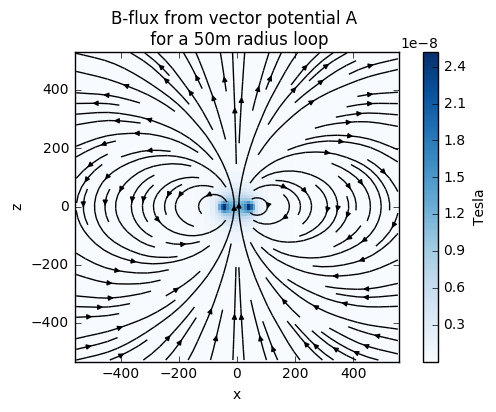
\includegraphics[scale=0.8]{./figures/initialisation/Bfield.png}
\caption{Static B flux}
\label{Static_B}
%\vspace{-40pt}
\end{figure}

We now need to define our initial condition for \textbf{b}. Here we are mostly interested to the response to a step-off function. We can then assume a magneto-static case at $t=0$ (see figure \ref{Static_B}).
Looking at the Ampere's equation (\ref{Ampere}), the magneto-static field generated by an inductive loop can be written as:
\begin{equation}
\nabla \times \mu_0^{-1}{\bf b} = \bf{j_s}
\end{equation}

The initialization for an inductive source is not dependent of the conductivity structures of the ground. Note this is not true for a galvanic source as in this case we would need first to solve the DC problem to get our source current term \cite{Haber:2014}. Also note that this would not be true either if we consider contrasts of magnetic permeability as this time we would need to formulate the problem using a fictitious source \cite{Haber:2014}.

Several options are now possible to solve the magneto-static problem for an inductive source. First there exists analytic solutions for \textbf{b} for a circular loop both for the magneto-static case and for the response to a step-off for an half-space. One might thinks this would be a wise choice here, since our goal is to implement different time-stepping methods, we need to compare them with an exact solution. However, if the exact continuous solution for \textbf{b} is divergence free as required, this is unlikely to be true for the discretized version on our domain. This will cause some major accuracy issues as presented in figure \ref{Convergence_Initialisation}, where we computed the response to a step-off of an half-space with our two types of initialization (script: TDEM\_initialization.py). To address that problem, since $\nabla \cdot {\bf b}=0$ by Gauss's law, we can express it in terms of a vector potential \textbf{a}:
\begin{equation}
{\bf b}= \nabla \times {\bf a}
\end{equation} 

The vector potential \textbf{a} is now a quantity that lives on the edges. It exists, as for \textbf{b}, an analytic solution for a circular loop. We can then compute it on every edges and use our discretized operator Curl to obtain a divergence-free discretized magnetic flux density \textbf{b}. However our initialization is no longer independent of our mesh and will have a quadratic convergence compared to the size of the cells (figures \ref{Init_p} \& \ref{Init_eps}), even if we use an analytic formulation for \textbf{a} (Script: Test\_convergence\_Initialization.py in the repository).

For any type of loop or even current distribution, it is also possible to initialize using an equivalent of the Biot-Savart's law for the vector potential \textbf{a}. This has also been implemented and will be useful for more general cases, as for example for square loops that are widely used on field.


\begin{figure}[!ht]
%\vspace{-10pt}
\centering
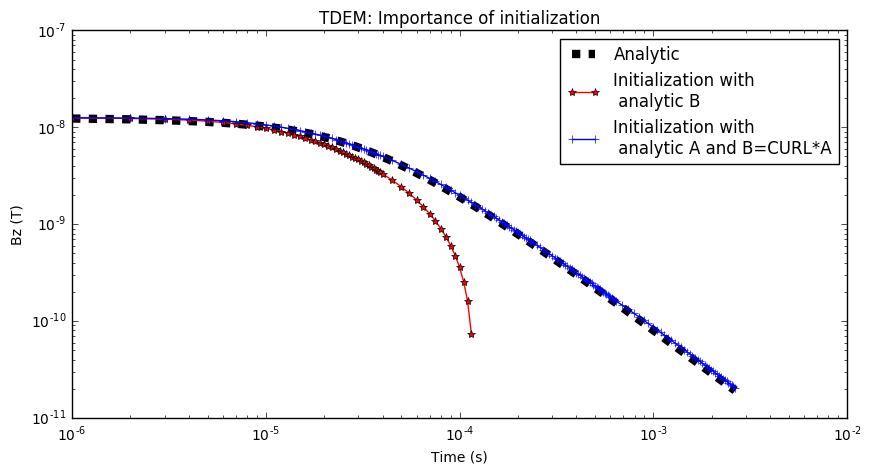
\includegraphics[scale=0.4]{./figures/initialisation/Initialization.png}
\caption{Accuracy with \textbf{a} or \textbf{b} initialization for an half-space,\\ all others parameters similar otherwise}
\label{Convergence_Initialisation}
%\vspace{-40pt}
\end{figure}

\begin{figure}[H]
\centering
\begin{minipage}{0.5\textwidth}
  \centering
  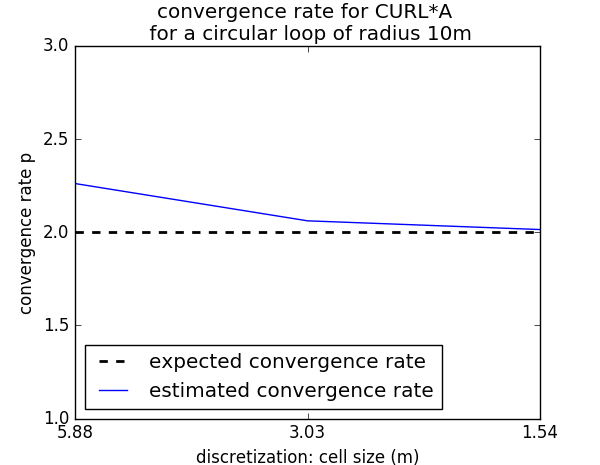
\includegraphics[width=.9\linewidth]{./figures/initialisation/ConvergenceRate_initialisation.png}
  \captionof{figure}{Initialization: Approximated convergence rate}
  \label{Init_p}
\end{minipage}%
\begin{minipage}{.5\textwidth}
  \centering
  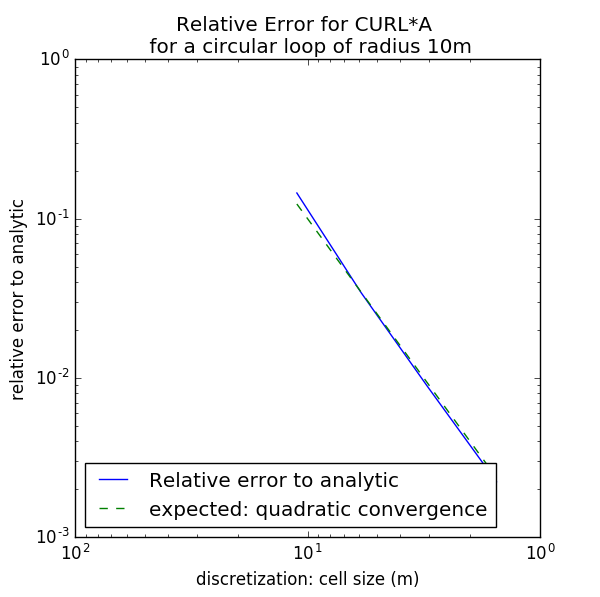
\includegraphics[width=.9\linewidth]{./figures/initialisation/relativeerror_Initialisation.png}
  \captionof{figure}{Initialization: Relative error \\ for a 10m radius loop}
  \label{Init_eps}
\end{minipage}
\end{figure}


\section{Meshing}

A crucial part of our problem (and still an open question for many aspects of it) is: how do we mesh? We are facing here several imperatives. First, we should discretize enough the loop and its interior such as our initial value is the best possible. Second, as the later we go in time, the further away the `smoke rings' are going and so should expand our mesh. Our cells should also be small enough to account update between our smaller expected time steps (at earliest times). Finally, our mesh should include the air as part of the model to avoid boundary conditions issues. This will be the case even when we refer to our model as an half-space (meant as an half-space homogeneous Earth).

These contradictory imperatives, small cell sizes on a large scales, have lead several authors to use specialized meshes such as Octree Meshes (\cite{Haber2007}) for large scale problems or cylindrical meshes (\cite{SimPEGEM}) to deal with layered Earth models or centered anomalies. For simplicity, we have here decided to only use a regular tensor mesh whose cells expand the further away from the core. This will nonetheless limit some of our abilities to test the mesh as the problem can become computationally expensive very quickly.

Telford and al. (\cite{Telford}) derive some formulas such as the speed of diffusion or diffusion distance (equivalent to the skin depth concept for plane wave) that can help to make decisions depending on the problem.

\section{Time Stepping}

\subsection{Quick stability analysis and stiffness}
Our initializations done, we can now begin to compute the response in time to the step-off. As the term ${\bf j}_s$ disappears, we now have:
\begin{align}
\frac{ \partial {\bf b}}{\partial t} & = -Curl~ M_{\sigma}^{e-1} Curl^T M_{\mu^{-1}}^f {\bf b} \label{PDE_B}\\
\frac{ \partial {\bf b}}{\partial t} & = L {\bf b}
\end{align}

Because $\nabla \cdot {\bf b}=0$, equation \ref{PDE_B} is very similar to the heat equation. In a full homogeneous space, $L=\sigma^{-1}\mu^{-1} \Delta$ and we would be able to write:
\begin{align}
\sigma \mu \frac{ \partial {\bf b}}{\partial t} & = \Delta {\bf b}
\end{align}

A quick absolute stability analysis in 1D assuming an uniform cell size \textit{h} gives that we need a time-step \textit{k} such that:
\begin{align}
k \leq \frac{\sigma \mu h^2}{2}
\end{align}

However, for most ground material, $\sigma \mu \simeq 10^{-8}$ (and $\sigma \mu \simeq 10^{-15}$ for the air),which make our problem very stiff. In our case, for diffusion phenomenons we are usually interested to a wide time window between $10^{-6}s$ and $10^{-1}s$ and our space discretization is in the order of $\simeq10m$. Moreover, for $t\leq10^{-7}$, our magneto-quasi-static assumption will not hold anymore and we would need to consider the wave behavior of Maxwell's equations. This make explicit method inadequate for most practical applications in our case. We thus decide to focus on implicit methods.

Our matrix operator \textbf{L} can be considered as a model-weighted Laplacian. As all our physical properties are positive, we are assure that all \textbf{L}'s eigenvalues are non-positive. This makes the use of A-stable implicit methods even more recommended.

We particularly focus here on the family of BDF methods, as they have a very stiff decay and thus damp quickly the high frequencies of the error due to the magneto-quasi-static approximation (\cite{HAO:2004}).

\subsection{Backward Euler}
The first of all these implicit methods is the well-known and widely used Backward Euler.

\begin{align}
{\bf b^{n+1}} = (I-kL)^{-1}{\bf b^n}
\end{align}

One drawback of implicit methods is they require to solve a linear system. By chance, the matrix is symmetric positive definite, which open a lot of possibilities for the choice of solver. We choose to use a direct solver designed to handle large sparse matrices, Pardiso (\cite{Pardiso1},\cite{Pardiso2},\cite{Pardiso3}), as we care here about the precision of our solution. It also keeps into memory the factorization, which speeds up the process as long as we keep the same time step. A conjugate gradient approach would have been another option from the side of iterative optimization methods.

One advantage of Backward Euler, and all the family of BDF methods, is that it damps the high frequencies. Also as this method is A-stable, we do not have to worry about stability.

This method has proven to be relatively resilient in term of meshing. Unadapted meshes did not seem to affect it as much as higher-order methods (see \textbf{5.3 BDF-2} section). We ran a convergence analysis with a loop at the surface of an half-space of conductivity $10^{-1} S/m$. The initial value is computed with a relative error of $0.37\%$ and we are focusing here on the accuracy for the mid-to-late time $10^{-4}s$, depending on how many time steps we are using to reach it (Script: Test\_convergence\_BackwardEuler\_TS.py). The convergence to the analytic solution is linear as expected (figure \ref{BE_p}). However as we can see on figure \ref{BE_eps}, with a regular time-step size, we still does not have an $99\%$ accuracy with 50 time steps. To diminish the number of time-steps, we can increase the time-step size at later times but we then have to re-factorize a new matrix to solve our linear system and similar accuracy is not ensured.

%It is important to note that we have observed, for all methods we have tested, that the accuracy of our time-step methods sometimes plateau at an accuracy of the same order of magnitude that our initial guess. 

\begin{figure}[!ht]
\centering
\begin{minipage}{0.5\textwidth}
  \centering
  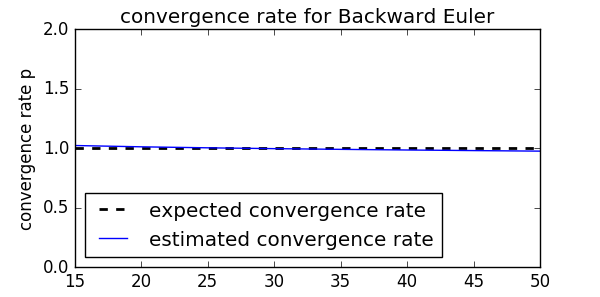
\includegraphics[width=.9\linewidth]{./figures/backwardEuler/ConvergenceRate_BE.png}
  \captionof{figure}{BE: Approximated convergence rate}
  \label{BE_p}
\end{minipage}%
\begin{minipage}{.5\textwidth}
  \centering
  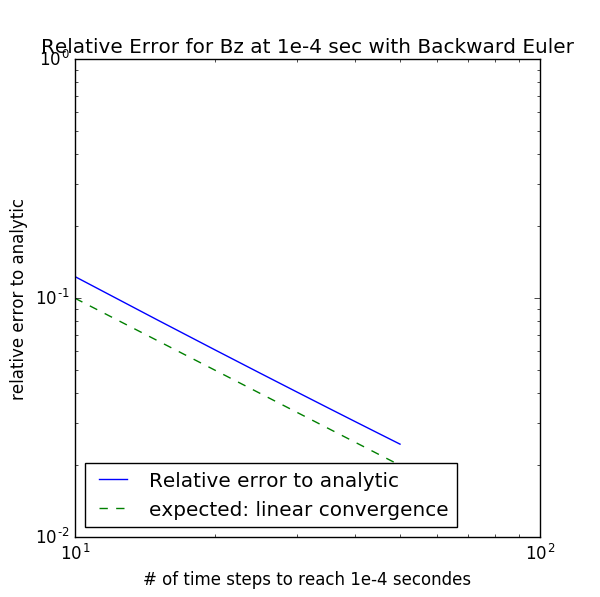
\includegraphics[width=.9\linewidth]{./figures/backwardEuler/relativeerror_BE_cs10_sig1e-1.png}
  \captionof{figure}{BE: Relative error}
  \label{BE_eps}
\end{minipage}
\end{figure}


\subsection{BDF-2}
We then use a BDF-2 scheme. This scheme first seemed appropriate as it has the same ability as backward Euler to damp high frequency modes and is an implicit scheme. It is using a polynomial interpolation between the different calculated states, which seemed reasonable as we are only observing the secondary field after the step-off (no source), which are known to be very smooth (see Maxwell's equations \ref{Faraday} \& \ref{Ampere} without source term).

\begin{align}
b^{n+1}= (I-\frac{2}{3}kL)^{-1}(\frac{4}{3} b^n - \frac{1}{3} b^{n-1})
\end{align}

We admit here our incapacity to perform a proper convergence analysis of this scheme (script: Test\_convergence\_BDF2\_TS.py). As it can be seen in figure \ref{Convergence_BDF2}, our scheme as here converge a lot more faster than expected. This has proven to be highly sensitive to our mesh, with sometimes convergence a bit less than expected for what we guess were unadapted meshes.
However in any cases we have observed, it has consistently displays better accuracy at late times than Backward Euler and in a lower number of time-steps for a comparable cost (compute the factorization of a similar matrix and then solve a right-hand-side for each time-step). For the same problem than the one solved previously with Backward Euler, we see here our relative error has damped to less than $1\%$ in less than 10 steps ($>50$ for Backward Euler) and up to a similar relative error than our initial state in about 20 steps. 

\begin{figure}[!ht]
%\vspace{-10pt}
\centering
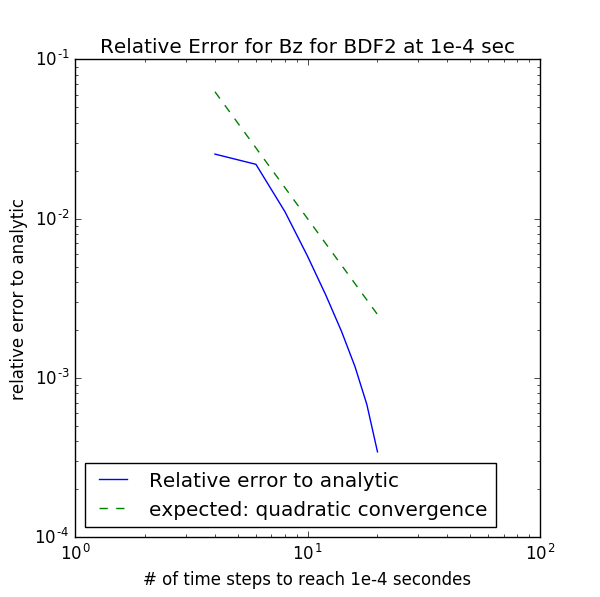
\includegraphics[scale=0.4]{./figures/BDF2/RelativeError_BDF2_morethanexpected_2.png}
\caption{Relative error for BDF2}
\label{Convergence_BDF2}
%\vspace{-40pt}
\end{figure}

Our best assumptions so far to explain our incapacity to compute a rate of convergence of 2 for BDF-2 are:
\begin{itemize}
\item As it is using a polynomial interpolation, the points where we evaluate it are important (our mesh)
\item We are converging too fast to a similar error than our initial state, not giving the time for the algorithm to stabilize
\item our intuition that the secondary fields are smoothed enough to be approximated by a polynomial is wrong
\end{itemize}

Another huge drawback of BDF-2 is that it cannot be used in a multiple steps sizes schemes as the coefficients assume a regular sampling in time (at least not without modifications to the coefficients, which would lead to Modified Divided Differences (\cite{krogh})). This can be problematic as usually data are recorded over several orders of magnitude of time (from $10^{-6}s$ to $10^{-1}s$). We would then recommend it as a fast way to get to late time and then switch to a Backward Euler scheme with various time-steps sizes.

\subsection{BDF-4}
We  only briefly tackled this method due to the challenges faced obtaining a proper convergence analysis of BDF-2. From the few tests we made, we generally obtained a very accurate result, better than BDF-2, in only 4 of 5 steps for late time. However it displays a tendency to lose accuracy as we increased the number of steps. Our best assumption is that, as this implicit method is no longer A-stable, we might have hit the instability region at some of the iterations.

\newpage
%------------------------------------------------

\section{Synthetic Examples}

\subsection{Half-Space}

Figure \ref{HS} and \ref{HS_eps} shows the computed response of an half-space of $\sigma = 10^{-1}s$ to a circular loop of $50m$ radius for both Backward Euler and BDF-2 and the obtained relative errors. Backward Euler is using an increasing time step starting at $10^{-6}s$ and updated every 100 steps, while BDF-2 is using a constant step size of $10^{-5}s$ (script: TDEM\_HalfSpace\_example.py)
For late time, BDF-2 is actually cheaper than Backward Euler, as we require to factorize a single matrix (for a single time step), whereas backward Euler need to re-factorize a new matrix each time we increase the time-step. We see that rapidly BDF-2 catch up and overcome Backward Euler for accuracy, even if it started later and with longer time steps. The loss of accuracy at later times for both methods can be explained by the size of the mesh as our eddy currents start being close to our boundaries. The bumps in Backward Euler are explained by the varying time-steps. However the `double picks' seen in BDF-2 for mid-to-late times ($\simeq 10^{-4}s$)is not completely understood but seems related to our increasing cell-sizes in our mesh (too fast or too soon increase?).

\begin{figure}[!ht]
\centering
\begin{minipage}{0.5\textwidth}
  \centering
  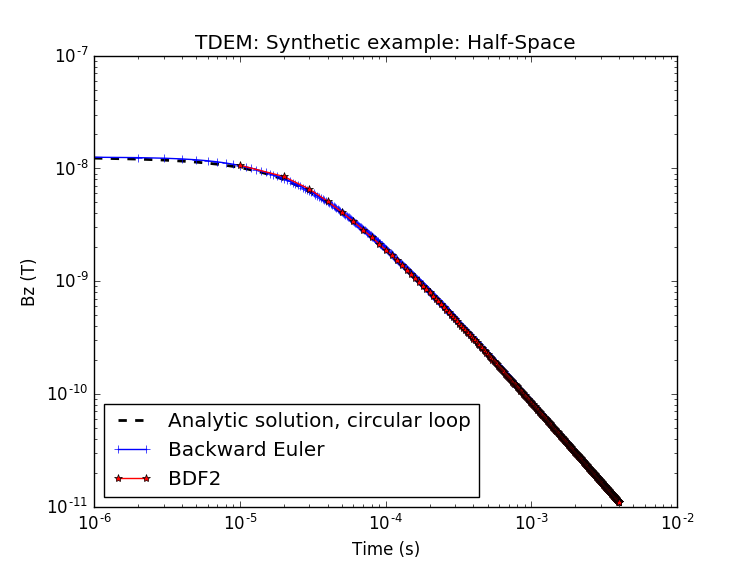
\includegraphics[width=.9\linewidth]{./figures/Examples/HalfSpace.png}
  \captionof{figure}{Half-Space Response: BE and BDF-2}
  \label{HS}
\end{minipage}%
\begin{minipage}{.5\textwidth}
  \centering
  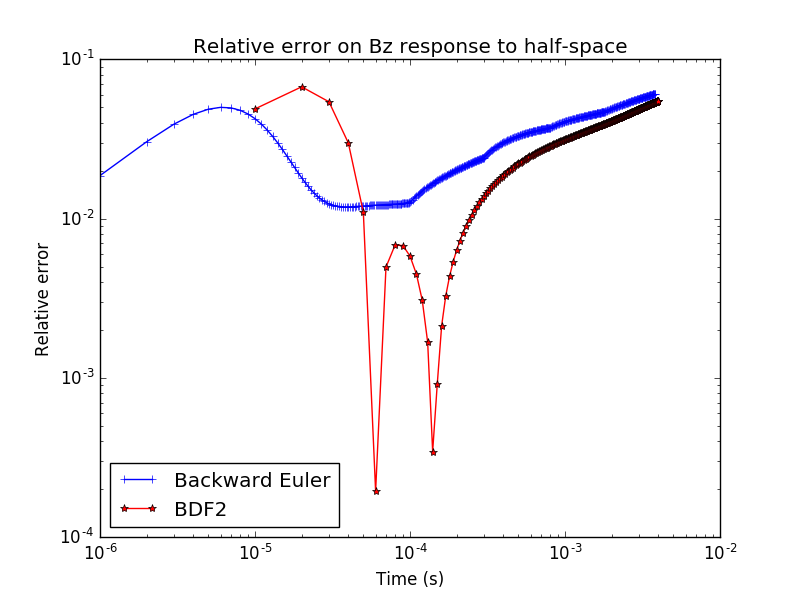
\includegraphics[width=.9\linewidth]{./figures/Examples/HS_relative_error.png}
  \captionof{figure}{Half-Space Response: BE and BDF-2 relative error}
  \label{HS_eps}
\end{minipage}
\end{figure}

\subsection{Layered Earth}

Finally, as a bonus to prove the abilities of our current code, consider a 2 layers Earth model (figure \ref{Layer_model}, the air is included for $z>0m$) of different conductivities with a square inductive loop at the surface (figure \ref{Square_loop}). Initialization is performed using a Biot-Savart's law for the vector potential \textbf{a} and computing the Curl of it to obtain the magnetic flux density ${\bf b}_0 = Curl~{\bf a}$ at $t=0$.

We then use a Backward Euler scheme to compute the model response to a step-off (see figure \ref{Layer_response}) with a multi-step-sizes strategy. In dashed, we compares our solution to the analytic for 2 homogeneous Earth with the same conductivity of each layer respectively induced by a circular inductive loop of same magnetic dipole moment as our square loop. We see very well that at early times we are only seeing the first layer and at later time we get closer and closer to the response of an homogeneous Earth composed only of the second layer. 

Figure \ref{Layer_eps} show the magnetic flux density at the last computed time. We can recognize well the anticipated diffusive `smoke ring'.

\begin{figure}[H]
\centering
\begin{minipage}{0.5\textwidth}
  \centering
  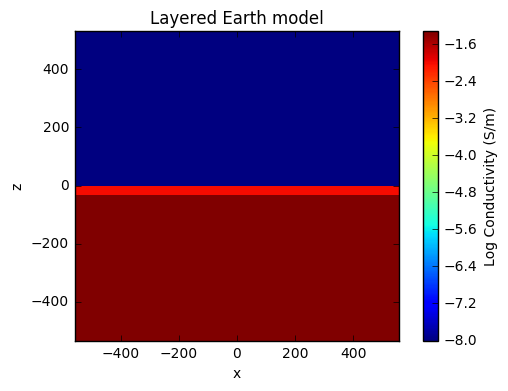
\includegraphics[width=\linewidth]{./figures/Examples/layerearthmodel.png}
  \captionof{figure}{Layered Earth Model}
  \label{Layer_model}
\end{minipage}%
\begin{minipage}{.5\textwidth}
  \centering
  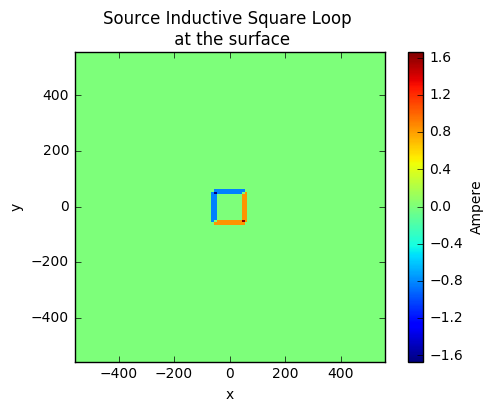
\includegraphics[width=\linewidth]{./figures/Examples/Source.png}
  \captionof{figure}{B-flux at the final time}
  \label{Square_loop}
\end{minipage}
\end{figure}

\begin{figure}[!ht]
\centering
\begin{minipage}{0.5\textwidth}
  \centering
  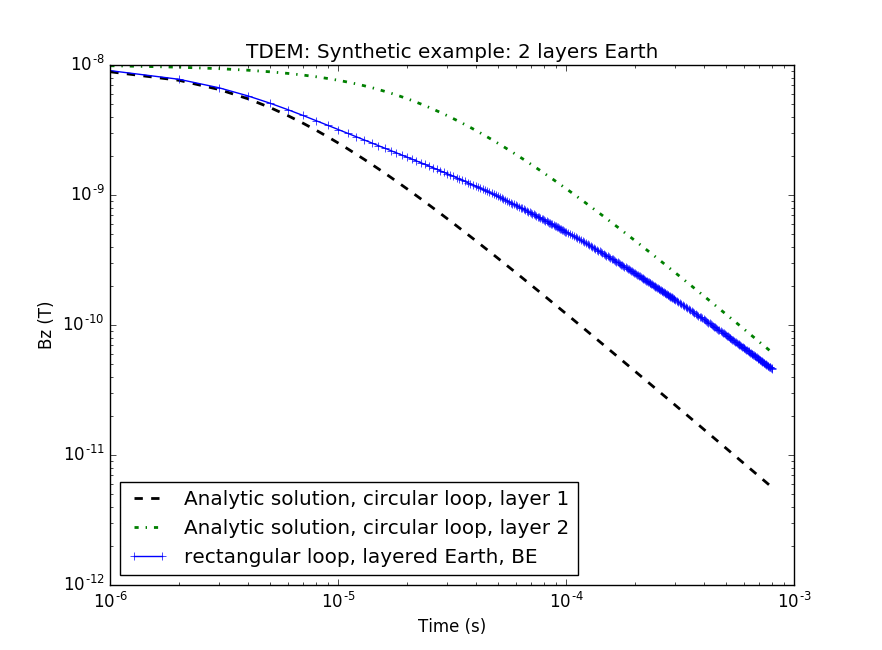
\includegraphics[width=\linewidth]{./figures/Examples/layerEarth_1em2_1em1p5_r55.png}
  \captionof{figure}{2-Layers Earth Response: \\ Backward Euler}
  \label{Layer_response}
\end{minipage}%
\begin{minipage}{.5\textwidth}
  \centering
  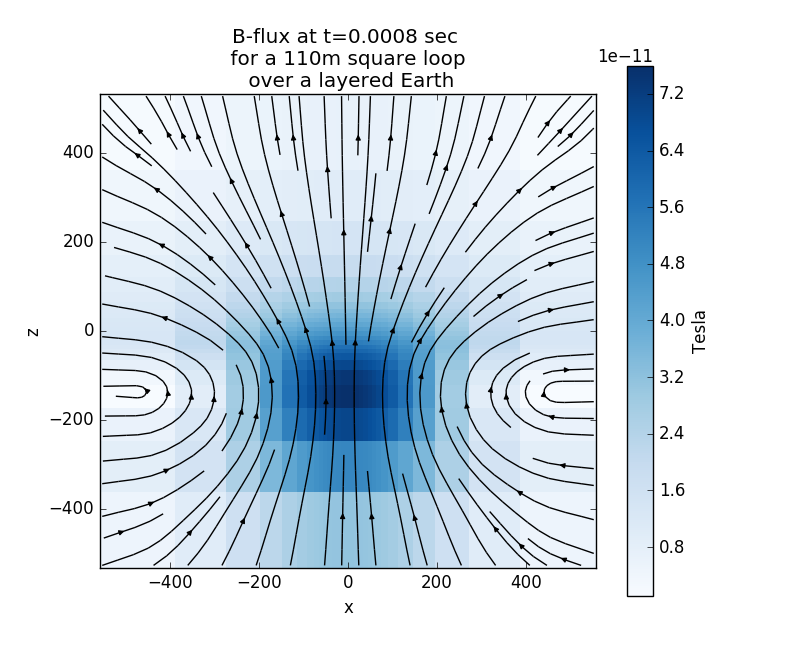
\includegraphics[width=\linewidth]{./figures/Examples/Field_layerEarth_1em2_1em1p5_r55.png}
  \captionof{figure}{B-flux at the final time}
  \label{Layer_eps}
\end{minipage}
\end{figure}

\newpage

\section{Discussion and conclusion}
We have built here a code that is able to forward model electromagnetic fields in time in response to a step-off for any discretized subsurface and survey configurations. Despite not addressed here, our code should also be able to deal with waveforms, as we are able to form our vector ${\bf j}_s$ and to include it in our matrices operators.

Initialization with a vector potential has been a key ingredient to the success of the code, as it ensures a divergence-free starting point.

Backward Euler is still the most widely used method in the domain for TDEM problems. It has proven, again, its reliability. BDF-2, despite failing to obtain a proper convergence analysis of our code, has given consistently more accurate results in less time steps and for a similar or even lower cost.

TDEM is a very stiff problem, with a lot of contradictory imperatives for the mesh that make the problem computationally expensive very quickly. Our time-steps, especially BDF-2, has shown unexpected behaviors associated with what we would guess being unadapted meshes for the problem. For further studies, it would be interesting to apply the same approach with a more efficient mesh in order to span more rigorously the space of variables (conductivity, cell size, mesh size...) and determine the key ingredients to an problem-adapted mesh that ensure a good behavior of the time-stepping methods.

Forward modeling is an important step of geophysics when it comes to invert data to recover a model. It is important to note that Backward Euler is usually easier to use as part of an inversion process. For late time interest, BDF-2 can be use in a strategic way combined to Backward Euler. It is in our opinion a very effective way to get close to the time windows of interest in few steps and we can then switch to a more appropriate time step size using Backward Euler.

%\section{Aknowlegdments}
%We look like to thanks Lindsey Heagy, Seogi Kang, Patrick Belliveau and Devin Cowan, all students at UBC - Geophysical Inversion Facility for sharing theirs experiences during the making of this project.
%----------------------------------------------------------------------------------------
%	REFERENCE LIST
%----------------------------------------------------------------------------------------
\newpage

\begin{thebibliography}{99}


\bibitem{CKH+:2015}
Cockett, Rowan, Seogi Kang, Lindsey J. Heagy, Adam Pidlisecky, and Douglas W. Oldenburg (2015)
\newblock "SimPEG: An Open Source Framework for Simulation and Gradient Based Parameter Estimation in Geophysical Applications." 
\newblock {\em Computers and Geosciences}, September 2015. doi:10.1016/j.cageo.2015.09.015.

\bibitem{krogh}
Krogh Fred T. (1974)
\newblock "Changing stepsize in the integration of differential equations using modified divided differences"
\newblock {\em Proceedings of the Conference on the Numerical Solution of Ordinary Differential Equations: 19,20 October 1972, The University of Texas at Austin}
\newblock pages="22-71, isbn= 978-3-540-37911-9, doi=10.1007/BFb0066584, url=http://dx.doi.org/10.1007/BFb0066584

\bibitem{HAO:2004}
Haber, E., U. Ascher, D. W. Oldenburg (2004).
\newblock "Inversion of 3D electromagnetic data in frequency and time using an inexact all-at-once approach"
\newblock {\em Geophysics}, vol. 69, 1216-1228.

\bibitem{Haber2007}
Haber, E., Heldmann S. (2007)
\newblock "An octree multigrid method for quasi-static Maxwell's equations with highly discontinuous coefficients"
\newblock {\em Journal of Computational Physics}, Volume 223 Issue 2, May, 2007, Pages 783-796

\bibitem{Haber:2014}
Haber E.(2014).
\newblock "Computational Methods in Geophysical Electrodynamics"

\bibitem{SimPEGEM}
Heagy J. lindsey, Rowan Cockett, Seogi Kang, Gudni K. Rosenkjaer, Douglas W. Oldenburg (2016)
\newblock "A framework for simulation and inversion in electromagnetics"
\newblock {\em Geophysics}

\bibitem{simpegjournal}
Heagy J. lindsey
http://simpeg.xyz/journal/dad772ba49ad31ddf3a3f7944511682b

\bibitem{Pardiso1}
Luisier M. , O. Schenk et.al. (2013)
\newblock Fast Methods for Computing Selected Elements of the Green's Function in Massively Parallel Nanoelectronic Device Simulations
\newblock Euro-Par 2013, LNCS 8097, F. Wolf, B. Mohr, and D. an Ney (Eds.), Springer-Verlag Berlin Heidelberg, pp. 533–544, 2013.

\bibitem{Nabighian}
Nabighian, M., and Macnae, J. (1991)
\newblock "Time domain electromagnetic prospecting methods, in Electromagnetic Methods in Applied Geophysics"
\newblock Volume 2: Application, Part A, chapter six,M. N. Nabighian (ed.), Society of Exploration Geophysicists, Tulsa, OK.

\bibitem{Pardiso2}
Schenk O., M. Bollhöfer, and R. Römer,
\newblock On large-scale diagonalization techniques for the Anderson model of localization.
\newblock Featured SIGEST paper in the SIAM Review selected "on the basis of its exceptional interest to the entire SIAM community". SIAM Review 50 (2008), pp. 91-112.

\bibitem{Pardiso3}
Schenk O., A. Wächter, and M. Hagemann,
\newblock Matching-based Preprocessing Algorithms to the Solution of Saddle-Point Problems in Large-Scale Nonconvex Interior-Point Optimization.
\newblock Journal of Computational Optimization and Applications, pp. 321-341, Volume 36, Numbers 2-3 / April, 2007.

\bibitem{Telford}
Telford, W.M., Geldart, L.P. and Sheriff, R.E. (1990)
\newblock Applied Geophysics, 2nd Edition: Cambridge University Press, 1990.

\bibitem{WH:1988}
S. H. Ward, C. W. Hohmann (1988).
\newblock "Electromagnetic Theory for Geophysical Applications", in Nabighian, M. N., Ed., Electromagnetic Methods in Applied Geophysics: Society of Exploration Geophysics.





\end{thebibliography}

%----------------------------------------------------------------------------------------

%\end{multicols}

\end{document}
